\section{Implementation}
\label{sec:implementation}

The abstract model of \name, optionally extended with a choosen set of
high-level consistency and isolation guarantees, can be instantiated
on top any eventually consistent key-value store. We now describe a
reference implementation of \name on top of Cassandra key-value
store~\cite{Cassandra}. Our implementation supports CV, CC, and SC
consistency levels (\S~\ref{sec:classification-scheme}) for data type
operations, and RC, MAV, and RR isolation levels
(\S~\ref{sec:isolation-guarantees}) for transactions. This
functionality is implemented entirely on top of the standard interface
exposed by Cassandra. From an engineering perspective, leveraging an
off-the-shelf data store enables an implementation comprising roughly
only 2500 lines of Haskell code, which is packaged as a
library~\cite{QueleaHackage}.

\subsection{Object State}

% http://www.planetcassandra.org/making-the-change-from-thrift-to-cql/

Cassandra adopts a data model similar to that of
BigTable~\cite{BigTable}. Each row is identified by a composite
\emph{primary key}, whose first component is the \emph{partition key},
and remaining components are \emph{clustering columns}. Like
Dynamo~\cite{Dynamo}, Cassandra uses consistent hashing on partition
key to map rows to machines in the cluster that maintain a replica.
Hence, rows with the same partition key (together referred to as a
\emph{partition}) are mapped to the same machine\footnote{Dynamo's
consistent hashing maps a partition key to a \emph{vnode}, which, in
common case, maps to a single physical machine.}. Within each
partition, rows are clustered and sorted on the values of their
clustering columns. \name relies on these properties to minize the
latency of querying object state stored in Cassandra.

Recall that the state of an object in \name is represented as a set of
effects. An effect generated as a result of executing an effectful
operation (eg.,\C{inc} or \C{withdraw}) inserts a new row
$(o,\allowbreak s,\allowbreak i, \allowbreak txn,\allowbreak val,
\allowbreak deps)$, where $o$ is the identifier of the object on which
the operation is perfomed, $s$ is the indentifier of the session that
issued the operation, and $i$ is operation's sequence number within
its session. The optional $txn$ column identifies the transaction (if
any). The column $val$ is the value associated with the effect (eg:
\cf{Withdraw 50}).  $deps$ is the set of identifiers of
\emph{dependencies} of this operation and is defined as $deps(e) =
\{e_1 \ALT \vis{e_1}{e} \wedge \neg(\exists e_2.\vis{e_1}{e_2} \wedge
\vis{e_2}{e})\}$. The primary key of this row is a composite of
$(o,s,i)$, making $o$ the partition key, and $s$ and $i$ clustering
columns. Thus, effects on same object belong to the same partition,
minizing the latency of reading its state. Within the partition,
effects are clustered (and sorted), first on $s$, then on $i$.
Consequently, range queries on $s$ and $i$, such as the set of effects
that precede a given effect in the same session (i.e., effects with
same $o$ and $s$, but lesser $i$), are efficient. This data model has
been crafted to enable efficient implementations of consistency
guarantees, such as session guarantees described in
\S~\ref{sec:classification-scheme}.

\subsection{Operation Consistency}

\begin{figure}
\begin{center}
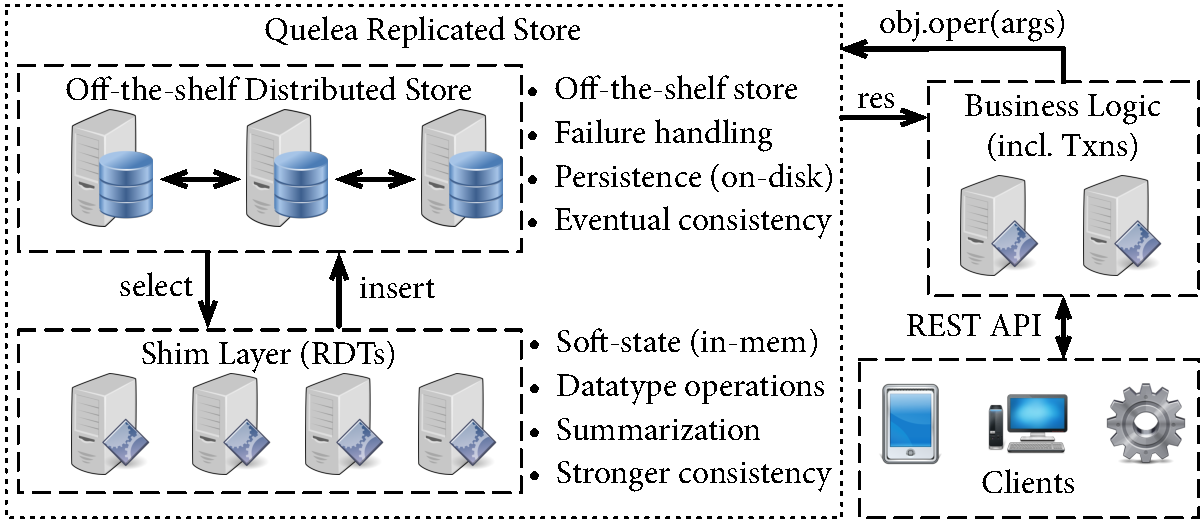
\includegraphics[width=\columnwidth]{Figures/ImplModel}
\end{center}
\caption{Implementation Model.}
\label{fig:impl_mod}
\end{figure}

The consistency semantics of replicated data types are implemented and
enforced in the \emph{shim layer} above Cassandra. The overall system
architecture is shown in Fig.~\ref{fig:impl_mod}. Note that shim layer
node simply acts as a soft-state write-through cache and can safely be
terminated at any point. Similarly, new shim layer nodes can be
spawned on demand.

The shim layer maintains a causal-visibility-consistent
(CV-consistent) in-memory state of a subset of objects in the system.
A CV-consistent state of an object is a subset of effects on the
object that are closed under the visibility relation.  In other words,
the shim layer includes an effect $e$ over an object $o$, only if it
also includes all effects $e'$ over $o$ that are visible to $e$ (i.e.,
$\vis{e'}{e}$). Since all read operations are served by the shim
layer, a read operation only ever witnesses CV-consistent state of its
object. Thus, CV consistency level is offered by default in this
implementation of \name.

The shim layer nodes periodically fetch updates from the backing
store, thereby ensuring that later operations witness more recent
CV-consistent state. For causally consistent operations, however,
updates need to be fetched on-demand. For example, if a causally
consistent operation $op$ on $o$ is the $i^{th}$ operation in session
$s$, and if the effect of ${i-1}^{th}$ operation in $s$ is not present
in the shim layer state of $o$, then a blocking read query for a row
with primary key $(o,s,i-1)$ needs to be issued by the shim layer.

Strongly consistent operations are performed after obtaining a
distributed global lock. Distributed lock can be implemented with the
help of Cassandra's conditional updates (lightweight transactions). To
prevent deadlocks due to crash failures of lock owner, the lock is
leased only for a pre-determined amount of time. Lease functionality
is implemented using Cassandra's support for and expiring columns.

\subsection{Transactions}

Multi-key coordination-free transactions are implemented in \name by
exploiting shim layer's default CV consistency guarantee. Recall that
the the shim layer does not include an effect unless all its
dependencies are also included. For every transaction, \name
instantiates a special transaction marker effect $m$ that is is
included as a dependence to every effect generated in the transaction.
Importantly, the marker $m$ is not inserted into the backing store
until and unless the transaction finishes execution. Now, any replica
which includes one of the effects from the transaction must include
$m$, and transitively must include every effect from the transaction.
This ensures atomicity and satisfies the RC requirement.

MAV semantics is implemented by keeping track of the set of
transaction markers $M$ witnessed by the transaction, and before
performing an operation at some replica, ensuring that $M$ is a subset
of the transaction markers included at that replica. If not, the
missing effects are synchronously fetched. RR semantics is realized by
capturing an optimized snapshot of the state of some replica; each
operation from an RR transaction is applied to this snapshot state.
Any generated effects are added to this snapshot.

\subsection{Summarization}

Observe that the state of an object in \name grows monotonically as
more effectful operations are performed on the object. Unbounded
growth of state makes querying prohibitively expensive at some point.
To keep the state in check, \name summarizes the object state both in
the shim layer node and the backing store, typically when the number
of effects on an object crosses a tunable threshold. \name's
summarization is similar in nature to the \emph{major compaction}
operation on \emph{SSTables} in BigTable.  While BigTable's compaction
summarizes reads and writes at the storage layer, \name summarizes
effects with application-specific semantics at the application layer.
Hence, semantics of summarization in \name is application-specific.
\name therefore requires its applications to implement a special
\cf{summarize} function that is called whenever the state needs to be
summarized. For example, bank account RDT's \cf{summarize} function
may summarize a state comprising multiple \cf{withdraw} and
\cf{deposit} effects into a single \cf{deposit} effect, thus
drastically reducing the number of effects that need to be kept track
of by the shim layer and the store.

